% Template for ASRU-2015 paper; to be used with:
%          spconf.sty  - ICASSP/ICIP LaTeX style file, and
%          IEEEbib.bst - IEEE bibliography style file.
% --------------------------------------------------------------------------
\documentclass{article}
\usepackage{spconf,amsmath,graphicx}
\usepackage{multirow}
\usepackage{caption,subcaption}
\usepackage{url}
\usepackage{hyperref}

% Example definitions.
% --------------------
\def\x{{\mathbf x}}
\def\L{{\cal L}}

% Title.
% ------
\title{Time delay deep neural network-based universal background models for speaker recognition\vspace{-2ex}}
%
% Single address.
% ---------------
\name{David Snyder, Daniel Garcia-Romero, Daniel Povey\vspace{-2ex}\thanks{This material is based upon work supported by the National Science Foundation Graduate Research Fellowship under Grant No. 1232825. Any opinion, findings, and conclusions or recommendations expressed in this material are those of the authors(s) and do not necessarily reflect the views of the National Science Foundation.}}
\address{Center for Language and Speech Processing \& Human Language Technology Center of Excellence\\
The Johns Hopkins University, Baltimore, MD 21218, USA\\
{\small \tt david.ryan.snyder@gmail.com, dgromero@jhu.edu, dpovey@gmail.com}}
%
% For example:
% ------------
%\address{School\\
%	Department\\
%	Address}
%
% Two addresses (uncomment and modify for two-address case).
% ----------------------------------------------------------
%\twoauthors
%  {A. Author-one, B. Author-two\sthanks{Thanks to XYZ agency for funding.}}
%	{School A-B\\
%	Department A-B\\
%	Address A-B}
%  {C. Author-three, D. Author-four\sthanks{The fourth author performed the work
%	while at ...}}
%	{School C-D\\
%	Department C-D\\
%	Address C-D}
%
\begin{document}
%\ninept
%
%\topmargin=-20mm
\maketitle
%
\begin{abstract}

Recently, deep neural networks (DNN) have been incorporated into i-vector-based speaker
recognition systems, where they have significantly improved state-of-the-art performance. In these
systems, a DNN is used to collect sufficient statistics for i-vector extraction.
In this study, the DNN is a recently developed time delay deep neural network
(TDNN) that has achieved promising results in LVCSR tasks. 
We believe that the
TDNN-based system achieves the best reported results on SRE10 and it obtains a 50\% relative 
improvement over our GMM baseline in terms of equal error rate (EER). 
For some applications, the computational cost of a DNN is high. 
Therefore, we also investigate a lightweight alternative in which a supervised GMM is derived from
the TDNN posteriors. This method maintains the speed of the traditional unsupervised-GMM,
but achieves a 20\% relative improvement in EER.
\end{abstract}
%
\begin{keywords}
speaker recognition, deep neural networks, time delay neural networks, i-vector
\end{keywords}
%
\vspace{12mm}
\section{Introduction}
\label{sec:intro}

Modern speaker recogntion systems are based on i-vectors \cite{ivector}.
In this paradigm, a universal background model (UBM) is used to collect
sufficient statistics for i-vector extraction, and a probabilistic 
linear discriminant analysis (PLDA) backend computes a similarity score between i-vectors
 \cite{plda_prince, brummer2010speaker, kenny2010bayesian, villalba2011towards, garcia2011analysis, garcia2012multicondition}.
Until recently, the state-of-the-art UBM was based on GMMs.

Recent speaker recognition systems have improved performance by replacing 
the GMM with a DNN to collect sufficient statistics (SS) for i-vector extraction \cite{lei2014, garcia2014}. 
Usually, this DNN is trained as the acoustic model in
an automatic speech recognition (ASR) system and is repurposed for
speaker recognition.
The output layer of a DNN provides soft alignments for
phonetic content, often tied triphone states (or senones). 
These DNN posteriors are used in conjunction with features extracted using a 
standard approach for speaker recognition, to create the sufficient statistics
for i-vector extraction \cite{ivector}.
The advantage of the DNN over the GMM may
be due to its ability to directly model phonetic content, rather than an arbitrary
acoustic space \cite{lei2014, garcia2014, kenny2014deep}. In \cite{garcia2014} it was found that
improvements to DNNs in terms of ASR word error rate (WER) may translate into 
improvements in speaker
recognition performance. Recently, recurrent neural networks (RNN) and TDNNs \cite{tdnn} have
outperformed traditional DNNs for a variety of LVCSR tasks \cite{lstm, saon2014, multisplice}.
In particular, the multisplice TDNN \cite{multisplice} had an 11\% WER
on Switchboard, better than RNN systems on the same task.
Our DNN is based on \cite{multisplice}. 

The DNN-based speaker recognition methods achieve excellent results, but the
performance comes at the cost of increased computational complexity. During
i-vector extraction, the role of the UBM is to produce frame-level posteriors.
For a DNN, the computation is nontrivial. In a resource limited application
that nonetheless requires realtime performance, the DNN-based system may
be impractical. Ideally, a supervised-GMM could be created with the 
speed of the traditional GMM-based UBM but with heightened phonetic awareness.
In \cite{omar2010} a GMM-based ASR acoustic model replaced the usual GMM-UBM
to create a phonetically aware GMM, but the improvements were only consistent
during model combination \cite{omar2010}.

Usually, DNN-based speaker recognition systems employ a supervised-GMM
derived from the DNN posteriors and speaker recognition features (often
not the same as the DNN features) \cite{lei2014, garcia2014, kenny2014deep}.
However, this GMM is not typically
used to collect SS; it has a minor role during i-vector extractor training.
Promoting this supervised-GMM to the role of the UBM was explored
in \cite{lei2014}, but it did not improve on their baseline.
It was speculated that this is due
to the GMM's limited ability to model phonetic information. However,
that GMM was diagonal, which possibly
reduced its modeling capacity. In this paper we reexamine the 
value of this supervised-GMM as a lightweight alternative to the DNN-based
speaker recognition system, and find that it consistently outperforms the
baseline.

\section{Experimental Setup}

\subsection{Datasets}
\label{datasets}
We evaluate our systems on the condition 5 extended task of 
SRE10 \cite{sre10}. The test consists of conversational telephone speech
in enrollment and test utterances. In total there are 416,119 trials,
over 98\% of which are nontarget comparisons. 

The UBM and i-vector extractor training data consists of male and female
utterances from SWB and NIST SREs prior to 2010. The SWB data contains
1,962 speakers and 20,905 utterances of SWB Cellular and SWB 2 
Phases II and III. The SRE dataset consists of 3,805 speakers 
and 36,614 utterances.
To create in-domain systems, the PLDA backends 
are trained only on the SRE data. About 1,800 hours
of the english portion of Fisher \cite{fisher} is
used to train the TDNN.

\subsection{DNN Recipe}
\label{dnn_recipe}

The system is based on the multisplice 
time delay DNN described
in \cite{multisplice}. This architecture is currently the recommended
recipe in the Kaldi toolkit \cite{kaldi} for large-scale speech recognition. 
In the multisplice system, a narrow temporal
context is provided to the first layer and increasingly wide
contexts are available to the subsequent hidden layers. The result is that
higher levels of the network are able to learn greater temporal
relationships. 

The features are 40 MFCCs without cepstral
truncation and with a frame-length of 25ms. 
These features are equivalent to filterbanks, but
are more compressible. Cepstral mean subtraction is 
performed over a window of
6 seconds. 

The TDNN has six layers, and a splicing configuration similar to those described
\cite{multisplice}. 
Suppose $t$ is some frame. At the input layer (layer 0)
frames $[t - 2, t + 2]$ are spliced together.
At layers 1, 3, and 4 we splice together frames 
$\{t-2, t+1\}$, $\{t - 3, t + 3\}$, and $\{t - 7, t + 2\}$, 
respectively.
In total, the DNN has a left-context of 13 and a right-context of 9.
The hidden layers use the $p$-norm (where $p=2$)
activation function \cite{pnorm}. The hidden layers have an 
input dimension of 350 and an output dimension 3500. 
The softmax output layer computes posteriors for 5297 triphone states. No
fMLLR or i-vectors are used for speaker adaptation.

\subsection{GMM-UBM Baseline}
\label{gmm_sys}

\begin{figure}[th]
\centerline{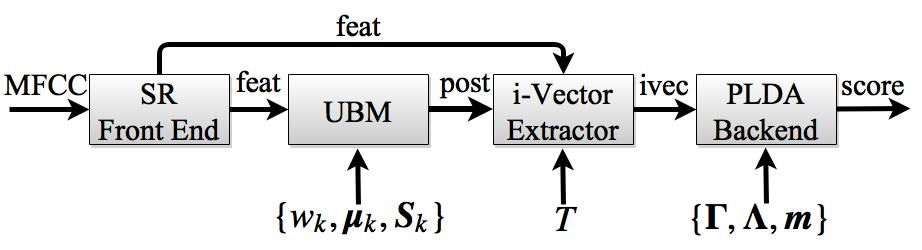
\includegraphics[width=8.5cm]{fig/baseline_schema}}
\caption{GMM-based speaker recognition schema.}
\label{fig:gmm_schema}
\end{figure}
The UBM in our baseline system (illustrated in Figure \ref{fig:gmm_schema})
is a full-covariance
GMM with several thousand mixture components. We compare
systems with 2048, 4096, and 5297 components. 
The front-end consists of 20 MFCCs with a 25ms frame-length.
The features are mean-normalized over a 3 second window. 
Delta and and acceleration are appended to create 60 dimensional
frame-level feature vectors. The nonspeech frames are then eliminated
using energy-based voice activity detection (VAD).

The GMM-UBM is trained on SWB and SRE datasets. It is initially trained
for 4 iterations of EM using a diagonal covariance matrix
 and then for an additional
4 iterations with a full-covariance matrix. A 600 dimensional i-vector
extractor is also trained on SWB and SRE for 5 iterations of EM.
The backend consists of i-vector mean subtraction and length
normalization, followed by PLDA scoring. To create an in-domain
system, we estimate the i-vector mean $\boldsymbol{m}$ and the 
between-class and within-class covariance matrices 
$\boldsymbol{\Gamma}$ and $\boldsymbol{\Lambda}$ of the PLDA backened 
using just the SRE dataset described in Section \ref{datasets}.

\subsection{Supervised GMM-UBM}
\label{sup_gmm_sys}

The goal of the supervised-GMM (shortened to sup-GMM) 
is to capture phonetic information
useful to speaker recognition in a lightweight model.
This is
achieved by creating a GMM based on DNN posteriors and speaker
recognition features. In contrast to the similar model in
 \cite{lei2014}, our sup-GMM is full-covariance. 
The supervised and unsupervised GMMs differ only
in the UBM training proceedure; during i-vector extraction,
both systems follow the diagram in Figure \ref{fig:gmm_schema}.

We use the TDNN described in Section \ref{dnn_recipe} to generate triphone posteriors on the SWB and SRE
training data. Speaker
recognition features (described in Section \ref{gmm_sys}) are also computed on this training data.
An energy-based VAD removes features and posteriors corresponding to nonspeech frames.

The mixture weights $w_{k}$, means $\boldsymbol{\mu}_{k}$ 
and covariances $\boldsymbol{S}_{k}$ are initialized according
to Equation (\ref{eq:sup_gmm_eq}). The DNN parameters are collectively
labeled $\boldsymbol{\Theta}$ and 
$Pr(k \mid \boldsymbol{y}_{i}, \boldsymbol{\Theta})$ is the
probability of triphone $k$ at frame $i$ given the DNN features $\boldsymbol{y}_{i}$. The
corresponding speaker recognition features are denoted $\boldsymbol{x}_{i}$.

\begin{equation}
\label{eq:sup_gmm_eq} 
\begin{split}
z_{k}^{(i)} &= Pr(k \mid \boldsymbol{y}_{i}, \boldsymbol{\Theta}), \\
w_{k} &= \sum_{i=1}^{N}z_{k}^{(i)},\\
\boldsymbol{\mu}_{k} &= \frac{1}{w_{k}} \sum_{i=1}^{N} z_{k}^{(i)} \boldsymbol{x}_{i},\\
\boldsymbol{S}_{k} &= \frac{1}{w_{k}} \sum_{i=1}^{N} z_{k}^{(i)} (\boldsymbol{x}_{i} - \boldsymbol{\mu}_{k}) (\boldsymbol{x}_{i} - \boldsymbol{\mu}_{k})^{\top}.
\end{split}
\end{equation}

Since the DNN output layer has 5297 senones, the sup-GMM also has 5297
components. 
Training of the $\boldsymbol{T}$ matrix
and PLDA parameters $\boldsymbol{\Gamma}$ and $\boldsymbol{\Lambda}$ are unchanged from Section \ref{gmm_sys}.

\subsection{TDNN-UBM}

\begin{figure}[th]
\centerline{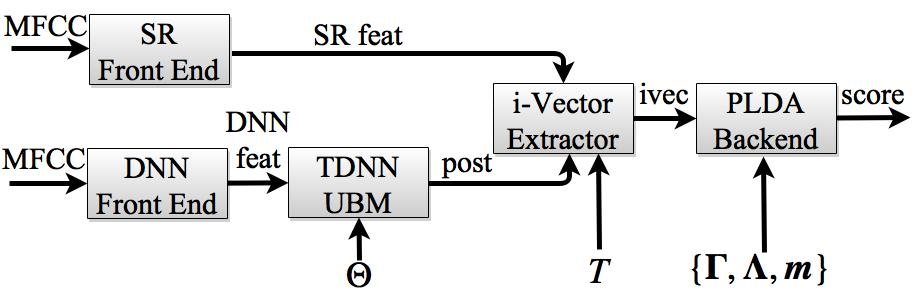
\includegraphics[width=8.5cm]{fig/dnn_schema}}
\caption{TDNN-based speaker recognition schema.}
\label{fig:dnn_schema}
\end{figure}

This system 
uses the TDNN of Section \ref{dnn_recipe} 
to create a UBM which directly models phonetic content.
This system is based on the in-domain system described in 
\cite{garcia2014} and is similar to
those in \cite{lei2014} and \cite{kenny2014deep}.
The primary difference between this and earlier work
is our utilization of the time delay DNN architecture.
The supervised-GMM (Section \ref{sup_gmm_sys}) fills the role
of the ancillary GMM of \cite{garcia2014}.
The parameters of the supervised-GMM 
are used to initalize quantities needed to train the
i-vector extractor $\boldsymbol{T}$ matrix. 

 
The only difference between this system and the preceding
GMM-based system is the model used to compute frame-level posteriors.
Here, TDNN posteriors and speaker recogntion features are used for both
i-vector extractor training and for computing enrollment and
test i-vectors.
The speaker recognition features are not the same as those used
by the DNN, as illustrated by the two 
feature pipelines in Figure \ref{fig:dnn_schema}.
 To maintain the correct temporal context,
an energy-based VAD is used to retain
just the posteriors and features corresponding to speech frames.
As in Sections \ref{gmm_sys} and \ref{sup_gmm_sys},
the i-vectors are 600 dimensional and the PLDA
backend is trained just on the in-domain SRE data.

\subsection{System Design}
Experiments used ASR and speaker recognition modules in the
Kaldi speech recognition toolkit \cite{kaldi}. Recipes for
the systems described here are available in the SRE10
example of the Kaldi code repository 
(\href{https://github.com/kaldi-asr/kaldi/tree/master/egs/sre10}{https://github.com/kaldi-asr/kaldi/tree/master/egs/sre10}).

\section{RESULTS}
\begin{table}
\begin{center}
\begin{tabular}{l|ccc}
\hline
System & EER(\%) & DCF$10^{-3}$ & DCF$10^{-2}$ \\ \hline \hline
Sup-GMM-5297 & 1.94 & 0.388 & 0.213 \\
TDNN-5297 & 1.20 & 0.216 & 0.123 \\
GMM-2048 & 2.49 & 0.496 & 0.288 \\
GMM-4096 & 2.56 & 0.468 & 0.287 \\
GMM-5297 & 2.42 & 0.484 & 0.290 \\ \hline
\end{tabular}
\end{center}
\caption{Performance comparison of gender independent models on SRE10 C5.}
\label{gender_ind}
\end{table}

\begin{table}
\begin{center}
\begin{tabular}{l|ccc}
\hline
System & EER(\%) & DCF$10^{-3}$ & DCF$10^{-2}$ \\ \hline \hline
Sup-GMM-5297 & 1.65 & 0.354 & 0.193 \\
TDNN-5297 & 1.09 & 0.214 & 0.108 \\
GMM-2048 & 2.16 & 0.417 & 0.239 \\
GMM-4096 & 1.96 & 0.414 & 0.227 \\
GMM-5297 & 2.00 & 0.410 & 0.241 \\ \hline
\end{tabular}
\end{center}
\caption{Performance comparison of gender dependent models on SRE10 C5.}
\label{gender_dep}
\end{table}

\begin{figure}[t]
\centerline{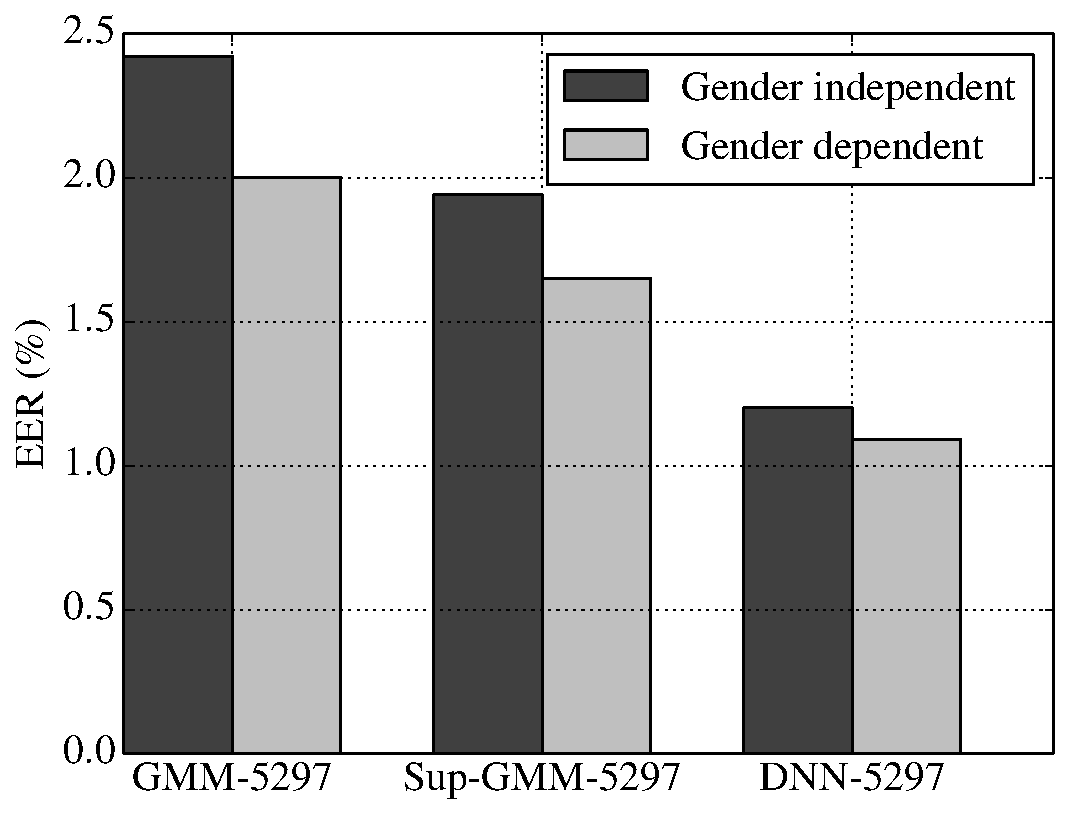
\includegraphics[width=8.5cm]{fig/eer}}
\caption{Comparison of EERs.}
\label{fig:eer}
\end{figure}

\begin{figure}[t]
\centerline{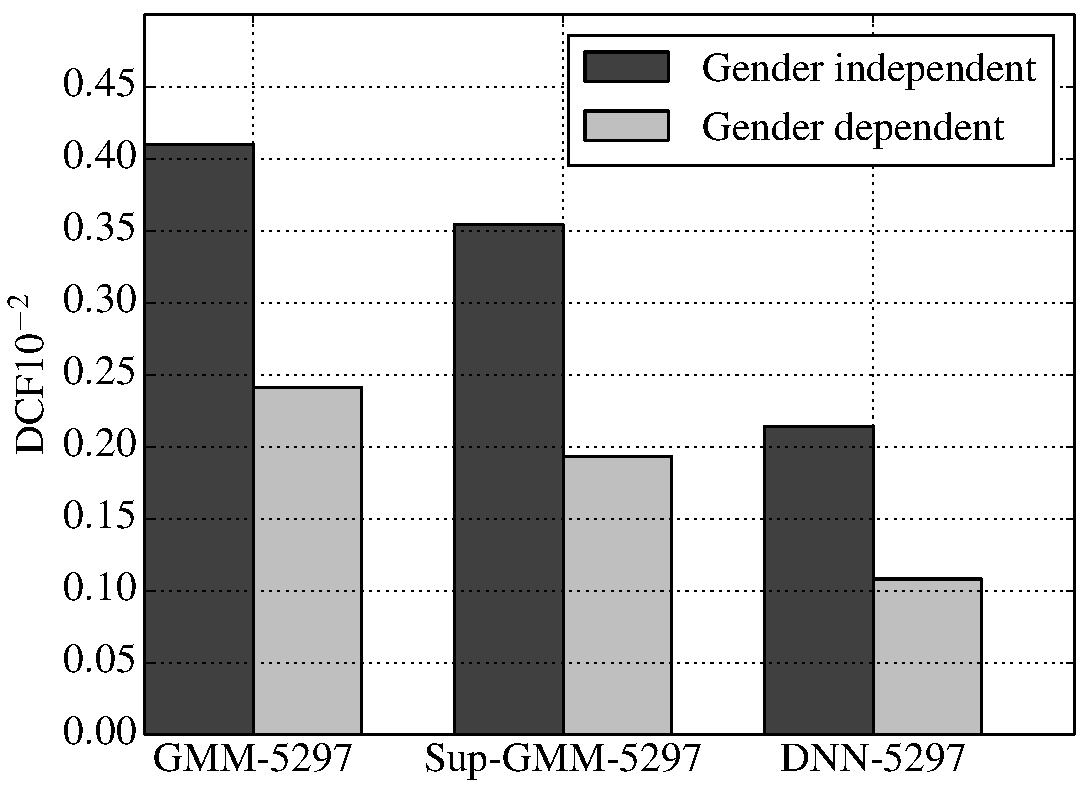
\includegraphics[width=8.5cm]{fig/dcf-2}}
\caption{Comparison of DCF$10^{-2}$.}
\label{fig:dcf_2}
\end{figure}

\begin{figure}[t]
\centerline{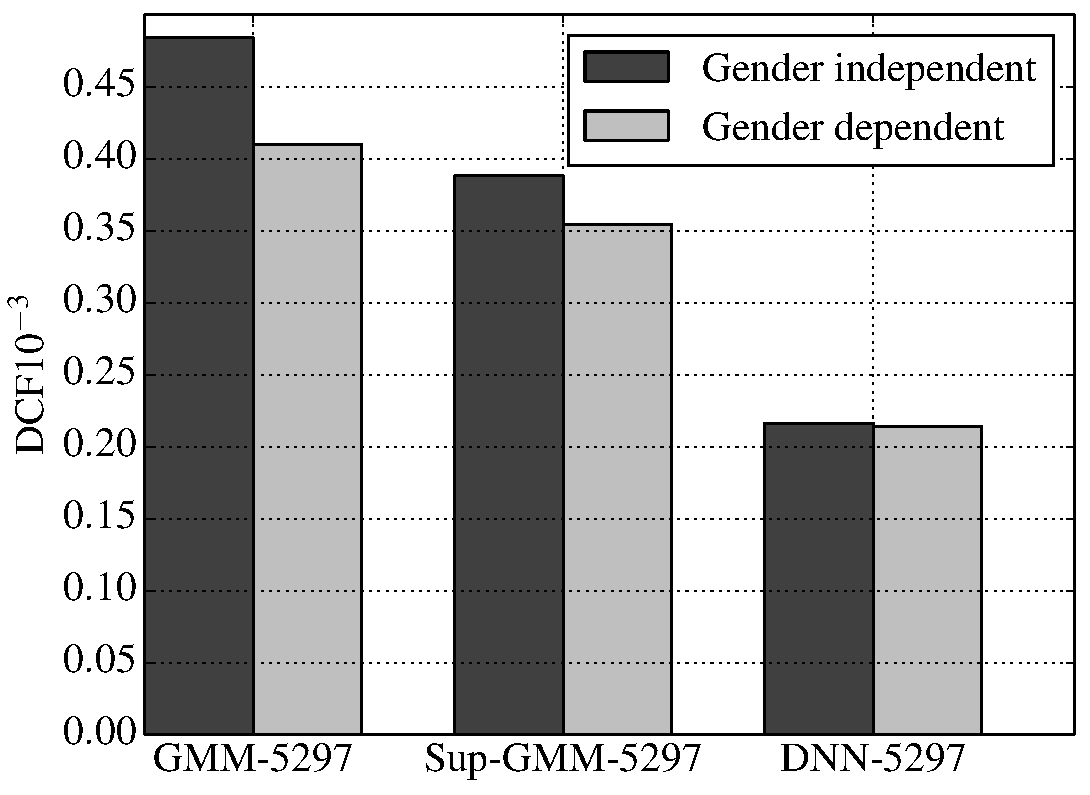
\includegraphics[width=8.5cm]{fig/dcf-3}}
\caption{Comparison of DCF$10^{-3}$.}
\label{fig:dcf_3}
\end{figure}

\begin{figure}[th]
\centerline{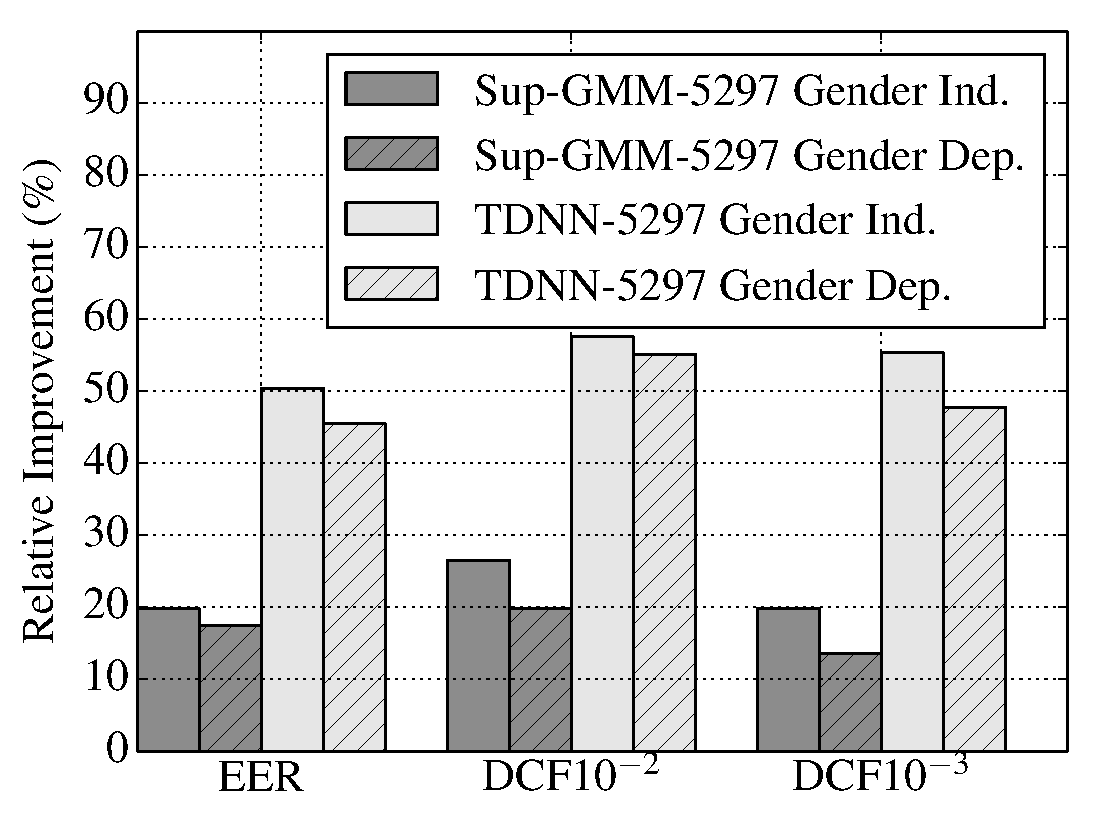
\includegraphics[width=8.5cm]{fig/rel}}
\caption{Relative improvement over
              the GMM-5297 baseline.}
\label{fig:rel}
\end{figure}

We compare gender independent and gender dependent versions of the
baseline GMM, sup-GMM and TDNN systems. The gender independent
systems each have a single pipeline which evaluates all of the SRE10
extended condition 5. The gender dependent systems share most of the
same components with the gender independent systems. 
The SRE data is partitioned into male and female sets and two PLDA
backends are trained. Accordingly, we evaluate the gender
dependent models on just the male or female portions of SRE10. To avoid 
overly large
tables we only report the performance for pooled gender dependent
and independent scores.
We evaluate recognition performance at three operating points: 
equal error-rate (EER) and normalized detection cost function (DCF) \cite{sre10}
with the probability of the target speaker set to $10^{-2}$ and $10^{-3}$.

In Tables \ref{gender_ind} and \ref{gender_dep} we see that there
isn't much of a performance difference between
the unsupervised GMMs with 2048, 4096 and 5297 components. 
We choose GMM-5297 as our primary baseline, since it has, 
by a small margin,
the best gender independent EER of the baseline models.

Figures \ref{fig:eer}, \ref{fig:dcf_2}, and \ref{fig:dcf_3}
compare the performance among the GMM-5297,
sup-GMM-5297 and TDNN-5297 systems. The DNN-based systems achieve the
best results, with TDNN-5297 obtaining 1.20\% and 1.09\%
gender independent and gender dependent EERs respectively.
Figure \ref{fig:rel} illustrates the relative improvement of the
TDNN and sup-GMM over the GMM-5297 baseline. Across the three
operating points with the gender independent and dependent systems we 
see a relative improvement of 13.65\%-26.55\%
by the sup-GMM and 47.80\%-57.59\% by the TDNN. Although
the performance of the sup-GMM isn't as good as the TDNN,
it nevertheless outperforms the baseline by a significant
margin. In similar methods such as \cite{lei2014} and \cite{omar2010}
the supervised-GMM did not result in a significant improvement by
itself. Perhaps the underlying reason lies in the high quality of
the TDNN which the sup-GMM is based on. Additionally, 
full-covariance may allow the sup-GMM to retain modeling capacity.

\begin{figure}[t]
\centerline{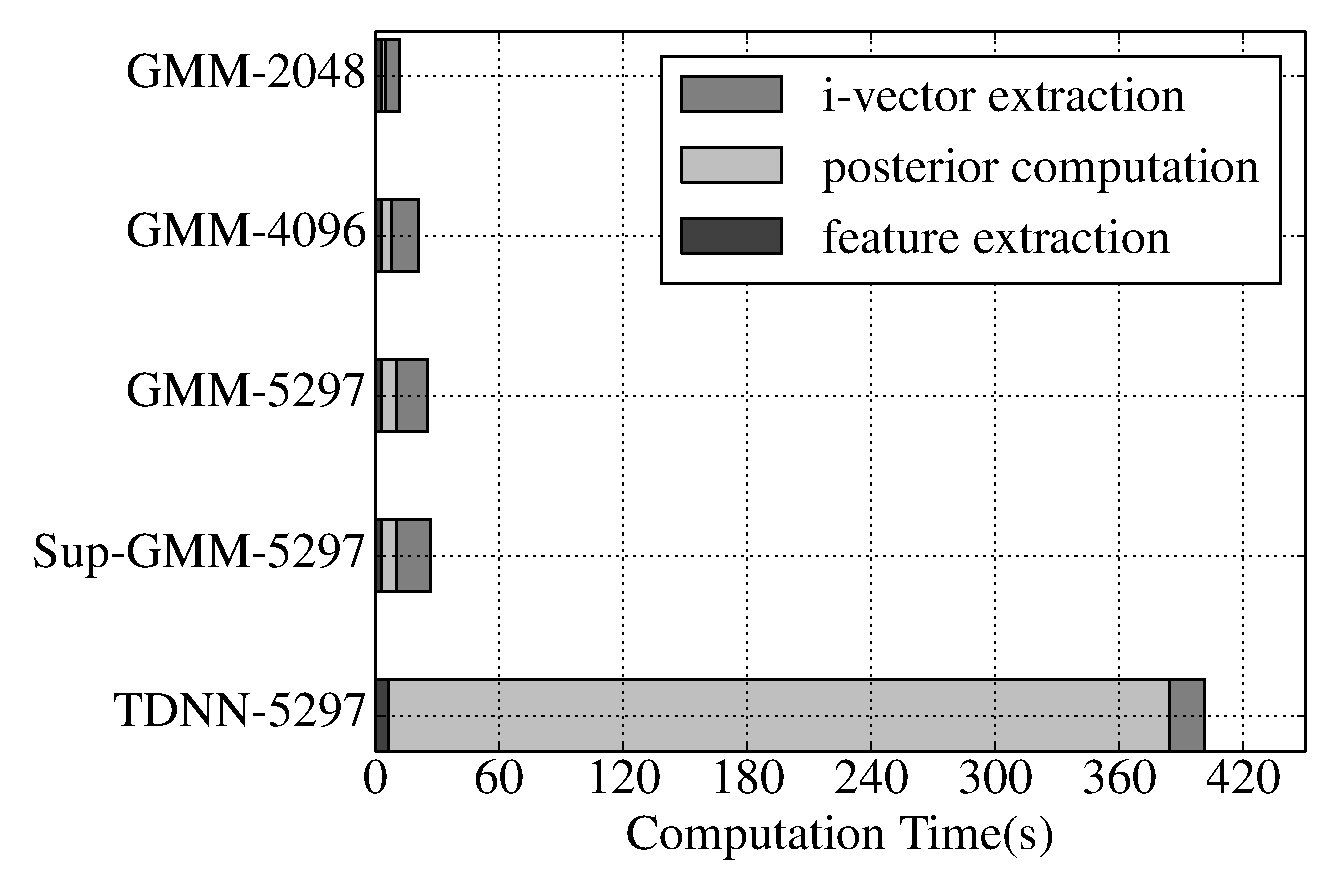
\includegraphics[width=8.5cm]{fig/time}}
\caption{Total CPU time relative to utterance length for each system.}
\label{fig:time}
\end{figure}

The primary advantage of a GMM-based method lies in its
efficiency during i-vector extraction. Using the sum of the \texttt{usr}
and \texttt{sys}
portions of the Linux tool \texttt{time} we recorded the duration of
different parts of the system pipelines. In Table \ref{timing} and
Figure \ref{fig:time}, we represent this in terms of real-time factors.
Ten 5 minute utterances
were selected at random from the SRE10 test data and these were processed
and timed from feature extraction to i-vector extraction 30 times. 
In Table \ref{timing} and
Figure \ref{fig:time}, i-vector extraction
includes all computation needed to generate an i-vector after posteriors and features
have been computed. The experiment was performed on an Intel x86-64 machine with 48 2000Mhz CPUs.
The real-time factors were obtained by taking the average durations In CPU and
dividing by the total utterance length. 

% TODO: Consider removing total. Note that the table is still too big
\begin{table}
\caption{CPU time relative to utterance length for primary stages of the system pipelines.}
\begin{center}
\begin{tabular}{l|ccc}
\hline
%System & Feat.(s) & Post.(s) & i-Vec.(s) & Tot.(s) \\ \hline \hline
%Sup-GMM-5297 & 3.05 & 10.39 & 16.32 & 29.76 \\
%TDNN-5297 & 6.46 & 384.05 & 17.30 & 407.81 \\
%GMM-5297 & 3.09  & 10.33 & 15.04 & 28.46 \\
%GMM-4096 & 3.04 & 8.00 & 12.82 & 23.86 \\
%GMM-2048 & 3.04 & 5.04 & 6.85 & 14.93 \\ \hline
System & Feat.(\%) & Post.(\%) & i-Vec.(\%)\\ \hline \hline
Sup-GMM-5297 & 1.02 & 3.46 & 5.44 \\
TDNN-5297 & 2.15 & 128.02 & 5.77  \\
GMM-5297 & 1.03 & 3.44 & 5.01 \\
GMM-4096 & 1.01 & 2.67 & 4.27 \\
GMM-2048 & 1.01 & 1.68 & 2.28 \\ \hline
\end{tabular}
\end{center}
\label{timing}
\end{table}


The GMM-2048 system is about twice as fast as the
larger GMMs with 4096 or 5297 components during posterior and i-vector
extraction. Even without
parallelization the GMM-based systems are at least ten times faster than
real-time. Since the TDNN system needs to compute features for both the
DNN and for speaker recognition, this stage of the pipeline is about twice
as slow as the GMM-based systems.
Without parallelization, the vast majority of the DNN-based system is spent 
in the posterior calculation. This results in a system which is nearly 36\% slower 
than real-time, and more than ten times slower than the sup-GMM-5297.

In practice we would perform the DNN posterior matrix calculations in
CUDA to obtain faster than real-time performance.
However, by comparing the total CPU time between the systems, we 
expose the overall computational load of the DNN, and facilitate
a comparison of compute-cost vs. performance of the three systems. 


%\begin{figure*}[!t]
%\centering
%  \begin{subfigure}[b]{0.49\textwidth}
%  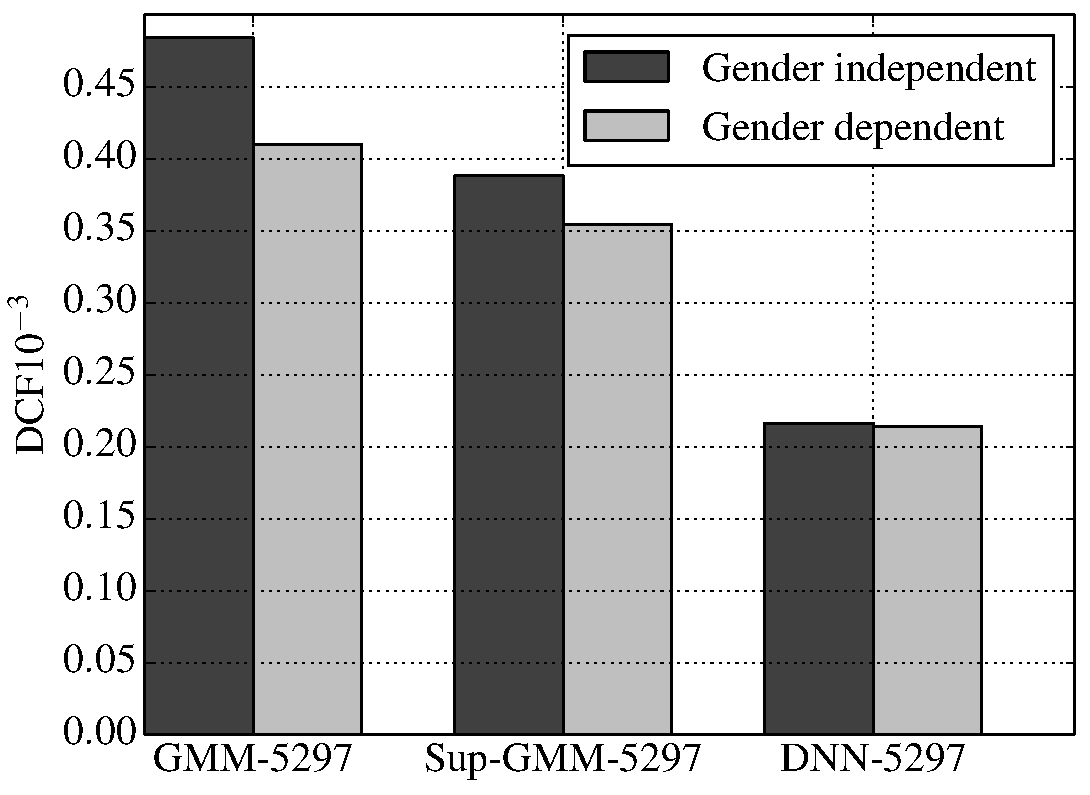
\includegraphics[width=8.5cm]{fig/dcf-3}     
%  \caption{}                           
%  \end{subfigure}
%  \begin{subfigure}[b]{0.49\textwidth}
%  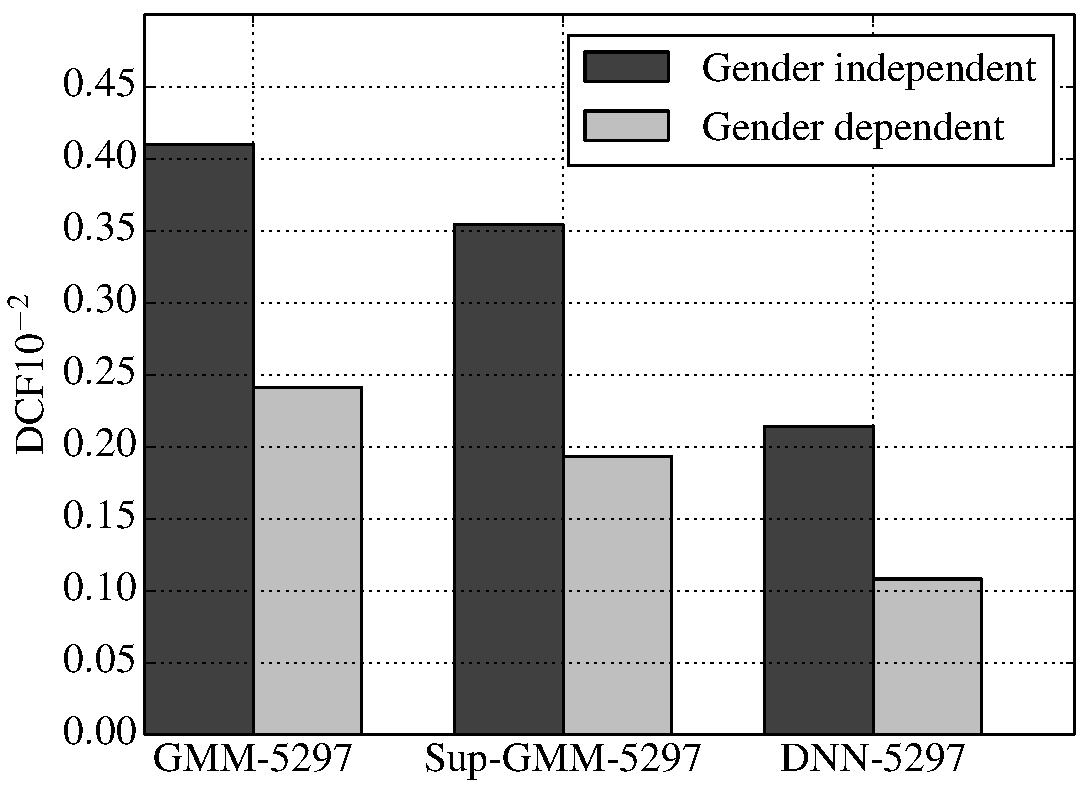
\includegraphics[width=8.5cm]{fig/dcf-2}   
%  \caption{}                                        
%  \end{subfigure}           
%  \caption{Performance on DCF with $10^{-3}$ and $10^{-2}$ operating points.}  
%  \label{fig:dcf}     
%\end{figure*}


%\begin{table}
%\begin{center}
%\begin{tabular}{l|ccc}
%\hline
%EER (\%) & Ind. Pool. & Ind. Fem. & Ind. Male \\ \hline \hline
%Sup-GMM & 1.94 & 1.98 & 1.79 \\
%DNN & 1.20 & 1.46 & 0.87 \\
%GMM-2048 & 2.49 & 2.35 & 2.51 \\
%GMM-4096 & 2.56 & 2.38 & 2.63 \\
%GMM-5297 & 2.42 & 2.43 & 2.40 \\ \hline
%\end{tabular}
%\end{center}
%\caption{EER on SRE10 C5 with gender independent models.}
%\label{eer_table}
%\end{table}
%
%\begin{table}
%\begin{center}
%\begin{tabular}{l|ccc}
%\hline
%EER (\%) & Dep. Pool. & Dep. Fem. & Dep. Male \\ \hline \hline
%Sup-GMM & 1.65 & 1.87 & 1.30 \\
%DNN & 1.09 & 1.43 & 0.72 \\
%GMM-2048 & 2.16 & 2.33 & 1.59 \\
%GMM-4096 & 1.96 & 2.14 & 1.41 \\
%GMM-5297 & 2.00 & 2.16 & 1.53 \\ \hline
%\end{tabular}
%\end{center}
%\caption{EER on SRE10 C5 with gender dependent models.}
%\label{eer_table}
%\end{table}

\section{Conclusion}

We explored the use of TDNNs for speaker recognition on the SRE10 task.
We found that this DNN yields a large relative improvement over the
unsupervised GMM baseline on EER and DCF operating points. With the
TDNN-UBM we also achieve a 1.20\% gender independent EER, 
which we believe is the best
reported on the task. We also highlighted the computational advantages
of the GMM over the DNN, and showed that there is a significant cost for
computing DNN posteriors. While GPU parallelization is commonly used to
obtain real-time performance, it may not be feasible for all applications.
We found that the supervised-GMM, normally
of minor use in the DNN-based system, can be 
used on its own as a fast alternative to the DNN with better performance
than the baseline. 

% References should be produced using the bibtex program from suitable
% BiBTeX files (here: strings, refs, manuals). The IEEEbib.bst bibliography
% style file from IEEE produces unsorted bibliography list.
% -------------------------------------------------------------------------
\bibliographystyle{IEEEbib}
\bibliography{refs}

\end{document}
